\documentclass{article}
\usepackage[backend=biber,natbib=true,style=alphabetic,maxbibnames=50]{biblatex}
\addbibresource{/home/nqbh/reference/bib.bib}
\usepackage[utf8]{vietnam}
\usepackage{tocloft}
\renewcommand{\cftsecleader}{\cftdotfill{\cftdotsep}}
\usepackage[colorlinks=true,linkcolor=blue,urlcolor=red,citecolor=magenta]{hyperref}
\usepackage{amsmath,amssymb,amsthm,float,graphicx,mathtools,tikz}
\usetikzlibrary{angles,calc,intersections,matrix,patterns,quotes,shadings}
\allowdisplaybreaks
\newtheorem{assumption}{Assumption}
\newtheorem{baitoan}{}
\newtheorem{cauhoi}{Câu hỏi}
\newtheorem{conjecture}{Conjecture}
\newtheorem{corollary}{Corollary}
\newtheorem{dangtoan}{Dạng toán}
\newtheorem{definition}{Definition}
\newtheorem{dinhluat}{Định luật}
\newtheorem{dinhly}{Định lý}
\newtheorem{dinhnghia}{Định nghĩa}
\newtheorem{example}{Example}
\newtheorem{ghichu}{Ghi chú}
\newtheorem{hequa}{Hệ quả}
\newtheorem{hypothesis}{Hypothesis}
\newtheorem{lemma}{Lemma}
\newtheorem{luuy}{Lưu ý}
\newtheorem{nhanxet}{Nhận xét}
\newtheorem{notation}{Notation}
\newtheorem{note}{Note}
\newtheorem{principle}{Principle}
\newtheorem{problem}{Problem}
\newtheorem{proposition}{Proposition}
\newtheorem{question}{Question}
\newtheorem{remark}{Remark}
\newtheorem{theorem}{Theorem}
\usepackage[left=1cm,right=1cm,top=5mm,bottom=5mm,footskip=4mm]{geometry}
\def\labelitemii{$\circ$}
\DeclareRobustCommand{\divby}{%
	\mathrel{\vbox{\baselineskip.65ex\lineskiplimit0pt\hbox{.}\hbox{.}\hbox{.}}}%
}
\def\labelitemii{$\circ$}

\title{Problem: Application of Derivative to Survey {\it\&} Draw Graph of Functions\\Bài Tập: Ứng Dụng Đạo Hàm Để Khảo Sát {\it\&} Vẽ Đồ Thị Của Hàm Số}
\author{Nguyễn Quản Bá Hồng\footnote{A Scientist {\it\&} Creative Artist Wannabe. E-mail: {\tt nguyenquanbahong@gmail.com}. Bến Tre City, Việt Nam.}}
\date{\today}

\begin{document}
\maketitle
\begin{abstract}
	This text is a part of the series {\it Some Topics in Elementary STEM \& Beyond}:
	
	{\sc url}: \url{https://nqbh.github.io/elementary_STEM}.
	
	Latest version:
	\begin{itemize}
		\item {\it Problem: Application of Derivative to Survey \& Draw Graph of Functions -- Bài Tập: Ứng Dụng Đạo Hàm Để Khảo Sát \& Vẽ Đồ Thị Của Hàm Số}.
		
		PDF: {\sc url}: \url{https://github.com/NQBH/elementary_STEM_beyond/blob/main/elementary_mathematics/grade_12/derivative_application/problem/NQBH_derivative_application_problem.pdf}.
		
		\TeX: {\sc url}: \url{https://github.com/NQBH/elementary_STEM_beyond/blob/main/elementary_mathematics/grade_12/derivative_application/problem/NQBH_derivative_application_problem.tex}.
		\item {\it Problem \& Solution: Application of Derivative to Survey \& Draw Graph of Functions -- Bài Tập \& Lời Giải: Ứng Dụng Đạo Hàm Để Khảo Sát \& Vẽ Đồ Thị Của Hàm Số}.
		
		PDF: {\sc url}: \url{https://github.com/NQBH/elementary_STEM_beyond/blob/main/elementary_mathematics/grade_12/derivative_application/solution/NQBH_derivative_application_solution.pdf}.
		
		\TeX: {\sc url}: \url{https://github.com/NQBH/elementary_STEM_beyond/blob/main/elementary_mathematics/grade_12/derivative_application/solution/NQBH_derivative_application_solution.tex}.
	\end{itemize}
\end{abstract}
\tableofcontents

%------------------------------------------------------------------------------%

\section{Monotonicity of Function -- Tính Đơn Điệu của Hàm Số}
\cite[Chap. I, \S1, pp. 5--14]{SGK_Toan_12_CD_tap_1}: HD1. LT1. LT2. HD2. LT3. LT4. HD3. HD4. LT5. 1. 2. 3. 4. 5. 6. 7.

\begin{dangtoan}
	Cho hàm số $y = f(x)$ có đồ thị như hình vẽ. Tìm khoảng đồng biến \& nghịch biến của hàm số $y = f(x)$.
\end{dangtoan}

\begin{proof}[Cách giải]
	Nhìn vào đồ thị, từ trái sang phải, khoảng nào hàm số $y = f(x)$ đi lên là khoảng đồng biến của hàm số $y = f(x)$, khoảng nào hàm số $y = f(x)$ đi xuống là khoảng nghịch biến của hàm số $y = f(x)$.
\end{proof}

\begin{baitoan}[\cite{TLCT_BT_dai_so_giai_tich_11}, 1., p. 54]
	Xét chiều biến thiên của hàm số: (a) $y = 4x^3 - 3x + 1$. (b) $y = \frac{1}{3}x^3 - \frac{5}{2}x^2 + 6x - 1$. (c) $y = \frac{1}{4}x^4 - 2x^3 + \frac{11}{2}x^2 - 6x + 2$. (d) $y = 3x + \frac{1}{x}$. (e) $y = x^2 + \dfrac{1}{x^2}$ (f) $y = \sqrt{1 - x^2}$. (g) $y = x\left(1993 + \sqrt{1995 - x^2}\right)$. (h) $y = \sqrt{2 + x - x^2}$.
\end{baitoan}

\begin{baitoan}[\cite{TLCT_BT_dai_so_giai_tich_11}, 2., p. 54]
	Chứng minh: (a) Hàm số $y = \dfrac{13x + 12}{22x + 12}$ nghịch biến trên từng khoảng xác định của nó. (b) Hàm số $y = \dfrac{2x^2 + 3x}{x + 1}$ đồng biến trên từng khoảng xác định của nó. (c) Hàm số $f(x) = \sqrt{4x^2 + 1} - 2x$ nghịch biến trên $\mathbb{R}$. (d) Hàm số $f(x) = x - \sin^2x$ đồng biến trên $\mathbb{R}$.
\end{baitoan}

\begin{baitoan}[\cite{TLCT_BT_dai_so_giai_tich_11}, 3., p. 54]
	Tìm tất cả $m\in\mathbb{R}$ để hàm số $y = f(x) = 3x^3 + mx^2 + x + 2$ đồng biến trên $\mathbb{R}$.
\end{baitoan}

\begin{baitoan}[\cite{TLCT_BT_dai_so_giai_tich_11}, 4., p. 54]
	Tìm tất cả $m\in\mathbb{R}$ để hàm số $y = f(x) = 3x + \dfrac{m}{x - 1}$ đồng biến trên từng khoảng xác định của nó.
\end{baitoan}

\begin{baitoan}[\cite{TLCT_BT_dai_so_giai_tich_11}, 5., p. 55]
	Chứng minh $\sin x\le x$ nếu $x\in[0,\infty)$, $\sin x > x$ nếu $x\in(-\infty,0)$.
\end{baitoan}

\begin{baitoan}[\cite{TLCT_BT_dai_so_giai_tich_11}, 6., p. 55]
	Chứng minh $\cos x\ge1 - \dfrac{x^2}{2}$, $\forall x\in\mathbb{R}$.
\end{baitoan}

\begin{baitoan}[\cite{TLCT_BT_dai_so_giai_tich_11}, 7., p. 55]
	Chứng minh $2\sin x + \tan x > 3x$, $\forall x\in\left(0,\frac{\pi}{2}\right)$.
\end{baitoan}

\begin{baitoan}[\cite{SGK_Toan_12_giai_tich_nang_cao}, VD1, p. 5]
	Chứng minh hàm số $f(x) = \sqrt{1 - x^2}$ nghịch biến trên đoạn $[0,1]$.
\end{baitoan}

\begin{baitoan}[\cite{SGK_Toan_12_giai_tich_nang_cao}, VD2, p. 6]
	Xét chiều biến thiên của hàm số $y = x + \dfrac{4}{x}$.
\end{baitoan}

\begin{baitoan}[\cite{SGK_Toan_12_giai_tich_nang_cao}, H1, p. 6]
	Xét chiều biến thiên của hàm số $y = \dfrac{1}{3}x^3 - \dfrac{3}{2}x^2 + 2x - 3$.
\end{baitoan}

\begin{baitoan}[\cite{SGK_Toan_12_giai_tich_nang_cao}, VD3, p. 6]
	Xét chiều biến thiên của hàm số $y = \dfrac{4}{3}x^3 - 2x^2 + x - 3$.
\end{baitoan}

\begin{baitoan}[\cite{SGK_Toan_12_giai_tich_nang_cao}, H2, p. 7]
	Xét chiều biến thiên của hàm số $y = 2x^5 + 5x^4 + \dfrac{10}{3}x^3 - \dfrac{7}{3}$.
\end{baitoan}

\begin{baitoan}[\cite{SGK_Toan_12_giai_tich_nang_cao}, 1., p. 7]
	Xét chiều biến thiên của hàm số: (a) $y = 2x^3 + 3x^2 + 1$. (b) $y = x^3 - 2x^2 + x + 1$. (c) $y = x + \dfrac{3}{x}$. (d) $y = x - \dfrac{2}{x}$. (e) $y = x^4 - 2x^2 - 5$. (f) $y = \sqrt{4 - x^2}$.
\end{baitoan}

\begin{baitoan}[\cite{SGK_Toan_12_giai_tich_nang_cao}, 2., p. 7]
	Chứng minh: (a) Hàm số $y = \dfrac{x - 2}{x + 2}$ đồng biến trên mỗi khoảng xác định của nó. (b) Hàm số $y = \dfrac{-x^2 - 2x + 3}{x + 1}$ nghịch biến trên mỗi khoảng xác định của nó.
\end{baitoan}

\begin{baitoan}[\cite{SGK_Toan_12_giai_tich_nang_cao}, 3., p. 8]
	Chứng minh các hàm số sau đây đồng biến trên $\mathbb{R}$: (a) $f(x) = x^3 - 6x^2 + 17x + 4$. (b) $f(x) = x^3 + x - \cos x - 4$.
\end{baitoan}

\begin{baitoan}[\cite{SGK_Toan_12_giai_tich_nang_cao}, 4., p. 8]
	Với giá trị nào của $a$ hàm số $y = ax - x^3$ nghịch biến trên $\mathbb{R}$?
\end{baitoan}

\begin{baitoan}[\cite{SGK_Toan_12_giai_tich_nang_cao}, 5., p. 8]
	Tìm các giá trị của tham số $a$ để hàm số $f(x) = \dfrac{1}{3}x^3 + ax^2 + 4x + 3$ đồng biến trên $\mathbb{R}$.
\end{baitoan}

\begin{baitoan}[\cite{SGK_Toan_12_giai_tich_nang_cao}, 6., p. 8]
	Xét chiều biến thiên của hàm số: (a) $y = \dfrac{1}{3}x^3 - 2x^2 + 4x - 5$. (b) $y = -\dfrac{4}{3}x^3 + 6x^2 - 9x - \dfrac{2}{3}$. (c) $y = \dfrac{x^2 - 8x + 9}{x - 5}$. (d) $y = \sqrt{2x - x^2}$. (e) $y = \sqrt{x^2 - 2x + 3}$. (f) $y = \dfrac{1}{x + 1} - 2x$.
\end{baitoan}

\begin{baitoan}[\cite{SGK_Toan_12_giai_tich_nang_cao}, 7., p. 8]
	Chứng minh hàm số $f(x) = \cos2x - 2x + 3$ nghịch biến trên $\mathbb{R}$.
\end{baitoan}

\begin{baitoan}[\cite{SGK_Toan_12_giai_tich_nang_cao}, 8., pp. 8--9]
	Chứng minh bất đẳng thức: (a) $\sin x < x$, $\forall x\in\mathbb{R}$, $x > 0$; $\sin x > x$, $\forall x\in\mathbb{R}$, $x < 0$. (b) $\cos x > 1 - \dfrac{x^2}{2}$, $\forall x\in\mathbb{R}$, $x\ne0$. (c) $\sin x > x - \dfrac{x^3}{6}$, $\forall x\in\mathbb{R}$, $x > 0$; $\sin x < x - \dfrac{x^3}{6}$, $\forall x\in\mathbb{R}$, $x < 0$.
\end{baitoan}

\begin{baitoan}[\cite{SGK_Toan_12_giai_tich_nang_cao}, 9., p. 9]
	Chứng minh: $\sin x + \tan x > 2x$, $\forall x\in\left(0,\dfrac{\pi}{2}\right)$.
\end{baitoan}

\begin{baitoan}[\cite{SGK_Toan_12_giai_tich_nang_cao}, 10., p. 9]
	Số dân của 1 thị trấn sau $t$ năm kể từ năm 1970 được ước tính bởi công thức $f(t) = \dfrac{26t + 10}{t + 5}$ ($f(t)$ được tính bằng nghìn người). (a) Tính số dân của thị trấn vào năm 1980 \& năm 1995. (b) Xem $f$ là 1 hàm số xác định trên nửa khoảng $[0,+\infty)$. Tìm $f'$ \& xét chiều biến thiên của hàm số $f$ trên nửa khoảng $[0,+\infty)$. (c) Đạo hàm của hàm số $f$ biểu thị tốc độ tăng dân số của thị trấn (tính bằng nghìn người{\tt/}năm). Tính tốc độ tăng dân số vào năm 1990 \& năm 2008 của thị trấn. Vào năm nào thì tốc độ tăng dân số là $0.125$ nghìn người{\tt/}năm?
\end{baitoan}

%------------------------------------------------------------------------------%

\section{Extremum of Function -- Cực Trị của Hàm Số}
Tìm cực trị của hàm số:

\begin{baitoan}[\cite{TLCT_BT_dai_so_giai_tich_11}, 8., p. 55]
	(a) $y = x^3 - 3x + 3$. (b) $y = -16x^3 + 3x^2 + 1$. (c) $y = 3x^4 - 4x^3 - 24x^2 + 48x - 3$. (d) $y = 2x + 1 + \dfrac{8}{x - 2}$.
\end{baitoan}

\begin{baitoan}[\cite{TLCT_BT_dai_so_giai_tich_11}, 9., p. 55]
	(a) $y = \dfrac{x^2 - 3x + 3}{x - 1}$. (b) $y = \dfrac{x}{x^2 + 2x + 4}$. (c) $y = x\sqrt{3 - x}$. (d) $y = x^2 - 4|x| + 3$.
\end{baitoan}

\begin{baitoan}[\cite{TLCT_BT_dai_so_giai_tich_11}, 10., p. 55]
	(a) $y = x\sqrt{4 - x^2}$. (b) $y = \sqrt{8 - x^2}$. (c) $y = x - \sin2x$. (d) $y = 3 - 2\cos x - \cos2x$.
\end{baitoan}

\begin{baitoan}[\cite{TLCT_BT_dai_so_giai_tich_11}, 11., p. 55]
	(a) $y = \sin^2x - \sqrt{3}\cos x$ với $x\in[0,\pi]$. (b) $y = 2\sin x + \cos2x$ với $x\in[0,\pi]$.
\end{baitoan}

\begin{baitoan}[\cite{TLCT_BT_dai_so_giai_tich_11}, 12., p. 55]
	Tìm 4 hệ số $a,b,c,d\in\mathbb{R}$ của hàm số $f(x) = ax^2 + bx^2 + cx + d$ để hàm số $f$ đạt cực tiểu tại điểm $x = 0$, $f(0) = 0$, \& đạt cực đại tại điểm $x = 1$, $f(1) = 1$.
\end{baitoan}

\begin{baitoan}[\cite{TLCT_BT_dai_so_giai_tich_11}, 13., p. 56]
	Tìm 4 hệ số $a,b,c,d\in\mathbb{R}$ sao cho hàm số $f(x) = x^3 + ax^2 + bx + c$ đạt cực tiểu tại điểm $x = 1$, $f(1) = -3$, \& đồ thị của hàm số cắt trục tung tại điểm có tung độ là $2$.
\end{baitoan}

\begin{baitoan}[\cite{TLCT_BT_dai_so_giai_tich_11}, 14., p. 56]
	Chứng minh $\forall m\in\mathbb{R}$, hàm số $y = \dfrac{x^2 - m(m + 1)x + m^3 + 1}{x - m}$ luôn có cực đại \& cực tiểu.
\end{baitoan}

%------------------------------------------------------------------------------%

\section{Maximum \& Minimum Values of Function -- Giá Trị Lớn Nhất \& Giá Trị Nhỏ Nhất của Hàm Số}
\cite[Chap. I, \S2, pp. 15--20]{SGK_Toan_12_CD_tap_1}: HD1. LT1. HD2. LT2. HD3. LT3. 1. 2. 3. 4. 5. 6. 7.

Tìm GTLN \& GTNN của hàm số:

\begin{baitoan}[\cite{TLCT_BT_dai_so_giai_tich_11}, 15., p. 56]
	(a) $f(x) = x^3 - 2x^2 + x + 1$ trên đoạn $[-3,3]$. (b) $f(x) = 5x^2 - 6x + 13$  trên đoạn $[0,2]$. (c) $f(x) = \dfrac{2x^2 + 3x + 1}{x + 2}$ trên đoạn $[-3,6]$. (d) $f(x) = x\sqrt{1 - x^2}$ trên đoạn $[-1,1]$. (e) $f(x) = x + 2 + \dfrac{1}{x - 1}$  trên khoảng $(1,\infty)$. (f) $f(x) = \dfrac{x^3}{x + 2}$  trên đoạn $[-1,2]$.
\end{baitoan}

\begin{baitoan}[\cite{TLCT_BT_dai_so_giai_tich_11}, 16., p. 56]
	(a) $f(x) = \sin^4x + \cos^4x$. (b) $f(x) = \sin^3x - \cos2x + \sin x + 2$. (c) $f(x) = \cos^22x - \sin x\cos x + 4$.
\end{baitoan}

\begin{baitoan}[\cite{TLCT_BT_dai_so_giai_tich_11}, 17., pp. 56--57]
	1 công ty bất động sản có $50$ căn hộ cho thuê. Biết nếu cho thuê mỗi căn hộ với giá $200000$ đồng{\tt/}tháng thì mọi căn hộ đều có người thuê \& cứ mỗi lần tăng giá cho thuê mỗi căn hộ $100000$ đồng{\tt/}tháng thì có thêm 2 căn hộ bị bỏ trống. Muốn có thu nhập cao nhất, công ty đó phải cho thuê mỗi căn hộ với giá bao nhiêu 1 tháng? Khi đó, có bao nhiêu căn hộ được cho thuê?
\end{baitoan}

\begin{baitoan}[\cite{TLCT_BT_dai_so_giai_tich_11}, 18., p. 57]
	1 hình chóp tứ giác đều ngoại tiếp hình cầu bán kính $a = {\rm const}$. Gọi $x$, $x > 2a$, là chiều cao của hình chóp. (a) Tính thể tích của hình chóp. (b) Tìm điều kiện của $x$ để hình chóp của thể tích nhỏ nhất.
\end{baitoan}

\begin{baitoan}[\cite{TLCT_BT_dai_so_giai_tich_11}, 19., p. 57]
	Cho hình thang cân $ABCD$ có đáy nhỏ $AB$ \& 2 cạnh bên đều dài {\rm1 m}. Tính $\alpha = \widehat{DAB} = \widehat{CBA}$ để hình thang có diện tích lớn nhất \& tính diện tích lớn nhất đó.
\end{baitoan}

\begin{baitoan}[\cite{TLCT_BT_dai_so_giai_tich_11}, 20., p. 57]
	Cho $\Delta ABC$ đều cạnh $a$. Dựng 1 hình chữ nhật $MNPQ$ có cạnh $MN$ nằm trên cạnh $BC$, 2 đỉnh $P,Q$ lần lượt nằm trên 2 cạnh $AC,AB$ của tam giác. Tìm vị trí của điểm $M$ sao cho hình chữ nhật có diện tích lớn nhất \& tìm {\rm GTLN} đó.
\end{baitoan}

\begin{baitoan}[\cite{TLCT_BT_dai_so_giai_tich_11}, 21., p. 57]
	Cho hàm số $f:\mathbb{R}\to\mathbb{R}$ thỏa $f(\cot x) = \sin2x + \cos2x$, $\forall x\in\mathbb{R}$. Tìm {\rm GTLN, GTNN} của hàm số $g(x) = f(x)f(1 - x)$ trên đoạn $[-1,1]$.
\end{baitoan}

\begin{baitoan}[\cite{SGK_Toan_12_giai_tich_nang_cao}, VD1, p. 14]
	Tìm cực trị của hàm số $f(x) = \dfrac{1}{3}x^3 - x^2 - 3x + \dfrac{4}{3}$.
\end{baitoan}

\begin{baitoan}[\cite{SGK_Toan_12_giai_tich_nang_cao}, H1, p. 14]
	Tìm cực trị của hàm số $f(x) = x + \dfrac{4}{x} - 3$.
\end{baitoan}

\begin{baitoan}[\cite{SGK_Toan_12_giai_tich_nang_cao}, VD2, p. 14]
	Tìm cực trị của hàm số $f(x) = |x|$.
\end{baitoan}

\begin{baitoan}[\cite{SGK_Toan_12_giai_tich_nang_cao}, VD3, p. 16]
	Tìm cực trị của hàm số $f(x) = \dfrac{1}{3}x^3 - x^2 - 3x + \dfrac{4}{3}$.
\end{baitoan}

\begin{baitoan}[\cite{SGK_Toan_12_giai_tich_nang_cao}, H2, p. 16]
	Tìm cực trị của hàm số $f(x) = 2\sin2x - 3$.
\end{baitoan}

\begin{baitoan}[\cite{SGK_Toan_12_giai_tich_nang_cao}, 11., pp. 16--17]
	Tìm cực trị của hàm số: (a) $f(x) = \dfrac{1}{3}x^3 + 2x^2 + 3x - 1$. (b) $f(x) = \dfrac{1}{3}x^3 - x^2 + 2x - 10$. (c) $f(x) = x + \dfrac{1}{x}$. (d) $f(x) = |x|(x + 2)$. (e) $f(x) = \dfrac{1}{5}x^5 - \dfrac{1}{3}x^3 + 2$. (f) $f(x) = \dfrac{x^2 - 3x + 3}{x - 1}$.
\end{baitoan}

\begin{baitoan}[\cite{SGK_Toan_12_giai_tich_nang_cao}, 12., p. 17]
	Tìm cực trị của hàm số: (a) $y = x\sqrt{4 - x^2}$. (b) $y = \sqrt{8 - x^2}$. (c) $y = x - \sin2x + 2$. (d) $y = 3 - 2\cos x - \cos2x$.
\end{baitoan}

\begin{baitoan}[\cite{SGK_Toan_12_giai_tich_nang_cao}, 13., p. 17]
	Tìm 4 hệ số $a,b,c,d\in\mathbb{R}$ của hàm số $f(x) = ax^3 + bx^2 + cx + d$ sao cho hàm số $f$ đạt cực tiểu tại điểm $x = 0$, $f(0) = 0$, \& đạt cực đại tại điểm $x = 1$, $f(1) = 1$.
\end{baitoan}

\begin{baitoan}[\cite{SGK_Toan_12_giai_tich_nang_cao}, 14., p. 17]
	Tìm 3 hệ số $a,b,c\in\mathbb{R}$ sao cho hàm số $f(x) = x^3 + ax^2 + bx + c$ đạt cực trị bằng $0$ tại điểm $x = -2$ \& đồ thị của hàm số đi qua điểm $A(1,0)$.
\end{baitoan}

\begin{baitoan}[\cite{SGK_Toan_12_giai_tich_nang_cao}, 15., p. 17]
	Chứng minh với mọi giá trị của $m$, hàm số $y = \dfrac{x^2 - m(m + 1)x + m^3 + 1}{x - m}$ luôn có cực đại \& cực tiểu.
\end{baitoan}

\begin{baitoan}[\cite{SGK_Toan_12_giai_tich_nang_cao}, VD1, p. 18]
	Tìm {\rm GTLN, GTNN} của hàm số $f(x) = \sqrt{4 - x^2}$.
\end{baitoan}

\begin{baitoan}[\cite{SGK_Toan_12_giai_tich_nang_cao}, VD2, p. 19]
	Tìm {\rm GTLN, GTNN} của hàm số $f(x) = x^3 - 3x + 3$ trên đoạn $\left[-3,\dfrac{3}{2}\right]$.
\end{baitoan}

\begin{baitoan}[\cite{SGK_Toan_12_giai_tich_nang_cao}, H, p. 19]
	Tìm {\rm GTLN, GTNN} của hàm số $f(x) = x + \dfrac{1}{x - 1}$ trên khoảng $(1,+\infty)$.
\end{baitoan}

\begin{baitoan}[\cite{SGK_Toan_12_giai_tich_nang_cao}, VD3, p. 20]
	1 hộp không nắp được làm từ 1 mảnh các tông theo mẫu như hình:
	\begin{figure}[H]
		\centering
		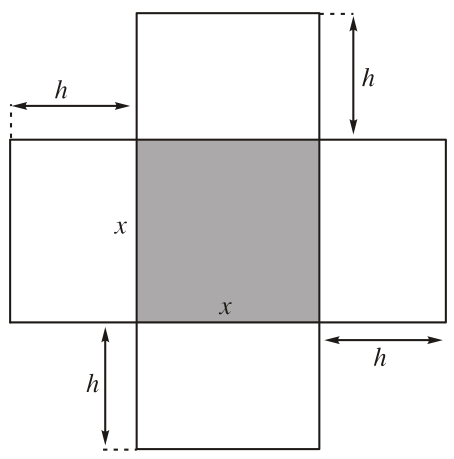
\includegraphics[scale=.25]{hop_khong_nap}
	\end{figure}
	\noindent Hộp có đáy là 1 hình vuông cạnh $x$ {\rm cm}, chiều cao là $h$ {\rm cm}, \& có thể tích là $500$ $\rm cm^3$. (a) Biểu diễn $h$ theo $x$. (b) Tìm diện tích $S(x)$ của mảnh các tông theo $x$. (c) Tìm giá trị của $x$ sao cho $S(x)$ nhỏ nhất.
\end{baitoan}

\begin{baitoan}[\cite{SGK_Toan_12_giai_tich_nang_cao}, VD4, p. 21]
	Tìm {\rm GTLN, GTNN} của hàm số $f(x) = x^3 - 3x + 3$ trên đoạn $[0,2]$.
\end{baitoan}

\begin{baitoan}[\cite{SGK_Toan_12_giai_tich_nang_cao}, 16., p. 22]
	Tìm {\rm GTLN, GTNN} của hàm số $f(x) = \sin^4x + \cos^4x$.
\end{baitoan}

\begin{baitoan}[\cite{SGK_Toan_12_giai_tich_nang_cao}, 17., p. 22]
	Tìm {\rm GTLN, GTNN} của hàm số: (a) $f(x) = x^2 + 2x - 5$ trên đoạn $[-2,3]$. (b) $f(x) = \dfrac{1}{3}x^3 + 2x^2 + 3x - 4$ trên đoạn $[-4,0]$. (c) $f(x) = x + \dfrac{1}{x}$ trên khoảng $(0,+\infty)$. (d) $f(x) = -x^2 + 2x + 4$ trên đoạn $[2,4]$. (e) $f(x) = \dfrac{2x^2 + 5x + 4}{x + 2}$ trên đoạn $[0,1]$. (f) $f(x) = x - \dfrac{1}{x}$ trên nửa khoảng $(0,2]$.
\end{baitoan}

\begin{baitoan}[\cite{SGK_Toan_12_giai_tich_nang_cao}, 18., p. 22]
	Tìm {\rm GTLN, GTNN} của hàm số: (a) $y = 2\sin^2x + 2\sin x - 1$. (b) $\cos^22x - \sin x\cos x + 4$.
\end{baitoan}

\begin{baitoan}[\cite{SGK_Toan_12_giai_tich_nang_cao}, 19., p. 22]
	Cho $\Delta ABC$ đều cạnh $a$. Dựng 1 hình chữ nhật $MNPQ$ có cạnh $MN$ nằm trên cạnh $BC$, 2 đỉnh $P,Q$ theo thứ tự nằm trên 2 cạnh $AC,AB$ của tam giác. Tìm vị trí của điểm $M$ sao cho hình chữ nhật có diện tích lớn nhất \& tìm {\rm GTLN} đó.
\end{baitoan}

\begin{baitoan}[\cite{SGK_Toan_12_giai_tich_nang_cao}, 20., p. 22]
	Khi nuôi cá thí nghiệm trong hồ, 1 nhà sinh vật học thấy: Nếu trên mỗi đơn vị diện tích của mặt hồ có $n$ con cá thì trung bình mỗi con cá sau 1 vụ cân nặng $P(n) = 480 - 20n$ {\rm g}. Hỏi phải thả bao nhiêu cá trên 1 đơn vị diện tích của mặt hồ để sau 1 vụ thu hoạch được nhiều cá nhất?
\end{baitoan}

\begin{baitoan}[\cite{SGK_Toan_12_giai_tich_nang_cao}, 21., p. 23]
	Tìm cực trị của hàm số: (a) $f(x)  = \dfrac{x}{x^2 + 1}$. (b) $f(x) = \dfrac{x^3}{x + 1}$. (c) $f(x) = \sqrt{5 - x^2}$. (d) $f(x) = x + \sqrt{x^2 - 1}$.
\end{baitoan}

\begin{baitoan}[\cite{SGK_Toan_12_giai_tich_nang_cao}, 22., p. 23]
	Tìm giá trị của $m$ để hàm số $f(x) = \dfrac{x^2 + mx - 1}{x - 1}$ có cực đại \& cực tiểu.
\end{baitoan}

\begin{baitoan}[\cite{SGK_Toan_12_giai_tich_nang_cao}, 23., p. 23]
	Độ giảm huyết áp của 1 bệnh nhân được cho bởi công thức $G(x) = 0.025x^2(30 - x)$, trong đó $x$ là liều lượng thuốc được tiêm cho bệnh nhân ($x$ được tính bằng {\rm mg}). Tính liều lượng thuốc cần tiêm cho bệnh nhân để huyết áp giảm nhiều nhất \& tính độ giảm đó.
\end{baitoan}

\begin{baitoan}[\cite{SGK_Toan_12_giai_tich_nang_cao}, 24., p. 23]
	Cho parabol $(\mathcal{P}):\ y = x^2$ \& điểm $A(-3,0)$. Tìm điểm $M$ thuộc parabol $(\mathcal{P})$ sao cho khoảng cách $AM$ là ngắn nhất \& tìm khoảng cách ngắn nhất đó.
\end{baitoan}

\begin{baitoan}[\cite{SGK_Toan_12_giai_tich_nang_cao}, 25., p. 23]
	1 con cá hồi bơi ngược dòng để vượt 1 khoảng cách là {\rm300 km}. Vận tốc dòng nước là {\rm6 km{\tt/}h}. Nếu vận tốc bơi của cá khi nước đứng yên là $v$ {\rm km{\tt/}h} thì năng lượng tiêu hao của cá trong $t$ giờ được cho bởi công thức $E(v) = cv^3t$, trong đó $c$ là 1 hằng số, $E$ được tính bằng jule. Tìm vận tốc bơi của cá khi nước đứng yên để năng lượng tiêu hao là ít nhất.
\end{baitoan}

\begin{baitoan}[\cite{SGK_Toan_12_giai_tich_nang_cao}, 26., pp. 23--24]
	Sau khi phát hiện 1 bệnh dịch, các chuyên gia y tế ước tính số người nhiễm bệnh kể từ ngày xuất hiện bệnh nhân đầu tiên đến ngày thứ $t$ là $f(t) = 45t^2 - t^3$, $t = 0,1,2,\ldots,25$. Nếu coi $f$ là hàm số xác định trên đoạn $[0,25]$ thì $f'(t)$ được xem là tốc độ truyền bệnh (người{\tt/}ngày) tại thời điểm $t$. (a) Tính tốc độ truyền bệnh vào ngày thứ 5. (b) Tìm ngày mà tốc độ truyền bệnh là lớn nhất \& tính tốc độ đó. (c) Tìm các ngày mà tốc độ truyền bệnh lớn hơn $600$. (d) Xét chiều biến thiên của hàm số $f$ trên đoạn $[0,25]$.
\end{baitoan}

\begin{baitoan}[\cite{SGK_Toan_12_giai_tich_nang_cao}, 27., p. 24]
	Tìm {\rm GTLN, GTNN} của hàm số: (a) $f(x) = \sqrt{3 - 2x}$ trên đoạn $[-3,1]$. (b) $f(x) = x + \sqrt{4 - x^2}$. (c) $f(x) = \sin^4x + \cos^2x + 2$. (d) $f(x) = x - \sin2x$ trên đoạn $\left[-\dfrac{\pi}{2},\pi\right]$.
\end{baitoan}

\begin{baitoan}[\cite{SGK_Toan_12_giai_tich_nang_cao}, 28., p. 24]
	Trong các hình chữ nhật có chu vi là {\rm40 cm}, xác định hình chữ nhật có diện tích lớn nhất.
\end{baitoan}

%------------------------------------------------------------------------------%

\section{Convexity \& Concavity of Graphs of Functions -- Tính Lồi Lõm \& Điểm Uốn của Đồ Thị}

\begin{baitoan}[\cite{TLCT_BT_dai_so_giai_tich_11}, 22., p. 57]
	Xét tính lồi, lõm của độ thị hàm số: (a) $y = x^3 - 3x^2 + x + 1$. (b) $y = -\frac{1}{3}x^3 - 2x^2 + 5$. (c) $y = x^4 - 5x^3 + x + 2$. (d) $y = -\frac{1}{4}x^4 + 3x^2 + x + 1$.
\end{baitoan}

\begin{baitoan}[\cite{TLCT_BT_dai_so_giai_tich_11}, 23., p. 57]
	Chứng minh mọi hàm đa thức bậc 3 đều có 1 điểm uốn \& điểm uốn đó chính là tâm đối xứng của đồ thị.
\end{baitoan}

\begin{baitoan}[\cite{TLCT_BT_dai_so_giai_tich_11}, 24., pp. 57--58]
	Giả sử $f$ là 1 liên tục trên khoảng $I$ thỏa $\dfrac{f(x) + f(y)}{2}\ge f\left(\dfrac{x + y}{2}\right)$, $\forall x,y\in I$. Chứng minh $f$ là hàm lõm trên $I$, i.e.,
	\begin{equation}
		(1 - \alpha)f(x) + \alpha f(y)\ge f((1 - \alpha)x + \alpha y),\ \forall x,y\in I,\,\alpha\in[0,1].
	\end{equation}
\end{baitoan}

\begin{baitoan}[\cite{TLCT_BT_dai_so_giai_tich_11}, 25., p. 58]
	Tìm $a,b\in\mathbb{R}$ để điểm $I(2,-6)$ là điểm uốn của đồ thị hàm số $y = ax^3 + bx^2 + x - 4$.
\end{baitoan}

\begin{baitoan}[\cite{TLCT_BT_dai_so_giai_tich_11}, 26., p. 58]
	Tìm $a\in\mathbb{R}$ để đồ thị hàm số $y = x^4 - ax^2 + 3$: (a) có 2 điểm uốn. (b) Không có điểm uốn nào.
\end{baitoan}

\begin{baitoan}[\cite{TLCT_BT_dai_so_giai_tich_11}, 27., p. 58]
	Chứng minh trong tất cả các tiếp tuyến với đồ thị hàm số $y = x^3 + 3x^2 - 9x + 5$, tiếp tuyến tại điểm uốn có hệ số góc nhỏ nhất.
\end{baitoan}

\begin{baitoan}[\cite{TLCT_BT_dai_so_giai_tich_11}, 28., p. 58]
	Chứng minh đồ thị hàm số $y = \dfrac{2x + 1}{x^2 + x + 1}$ có 3 điểm uốn thẳng hàng. Viết phương trình đường thẳng đi qua các điểm uốn.
\end{baitoan}

%------------------------------------------------------------------------------%

\section{Graph of a Function \& Some Graph Transformations -- Đồ Thị của Hàm Số \& 1 Số Phép Biến Đổi Đồ Thị}

\subsection{Graph of a function -- Đồ thị hàm số}
\fbox{1} {\sf Đồ thị hàm số}: Nếu $f$ là 1 hàm số có miền xác định $D$ (also $D_f,{\rm dom}(f)$) thì đồ thị hàm số $f$ là tập hợp các cặp sắp thứ tự $G_f\coloneqq\{(x,f(x));x\in D\}$, i.e., đồ thị của $f$ bao gồm tất cả các điểm $(x,y)$ trong mặt phẳng tọa độ $Oxy$ với $y = f(x)$ \& $x$ thuộc vào miền xác định của $f$; đôi khi cũng gọi đồ thị đó là 1 {\it đường cong} (curve), đặc biệt khi miền xác định là 1 khoảng, đoạn. \fbox{2} Trong mặt phẳng tọa độ $Oxy$, cho đồ thị $(G)$ của hàm số $y = f(x)$, $p,q\in(0,\infty)$. {\sf Phép tịnh tiến song song với trục tọa độ}: Tịnh tiến $(G)$ lên trên $q$ đơn vị được đồ thị hàm số $y = f(x) + q$, xuống dưới $q$ đơn vị được đồ thị hàm số $y = f(x) - q$, sang trái $p$ đơn vị được đồ thị hàm số $y = f(x + p)$, sang phải $p$ đơn vị được đồ thị hàm số $y = f(x - p)$. {\sf Phép đối xứng song song với trục tọa độ}: Nếu lấy hình đối xứng của $(G)$ qua trục $Oy$, được đồ thị hàm số $y = f(-x)$. Nếu lấy phần $(G^{\rm r})$ của $(G)$ nằm bên phải (right) của trục $Oy$ hợp với ảnh của $(G^{\rm r})$ qua phép đối xứng qua trục $Oy$, được đồ thị hàm số $y = f(|x|)$. Nếu lấy hình đối xứng của $(G)$ qua trục $Ox$, được đồ thị hàm số $y = -f(x)$. Nếu lấy phần $(G^{\rm a})$ của $(G)$ nằm bên trên (above) trục $Ox$ hợp với ảnh của $(G^{\rm b})$ -- phần của $(G)$ nằm bên dưới (below) trục $Ox$ -- qua phép đối xứng qua trục $Ox$, được đồ thị hàm số $y = |f(x)|$.

\begin{principle}[On graph transformations -- Về phép biến đổi đồ thị]
	Về mặt nguyên tắc, 1 hàm số bất kỳ có thể được khảo sát \& vẽ đồ thị theo 1 sơ đồ tổng quát. Nhưng đồ thị của các hàm số có mối liên quan đặc biệt có thể thu được từ nhau trực tiếp thông qua các phép biến đổi đồ thị, giúp rút ngắn thời gian thực hiện cũng như cho phép ta nhìn các đồ thị trong 1 mối tương quan thống nhất chứ không phải là các đối tượng riêng lẻ.
\end{principle}

\begin{baitoan}
	Trong mặt phẳng tọa độ $Oxy$: (a) Hình thu được qua phép đối xứng tâm $M(a,b)$, với $a,b\in\mathbb{R}$, của đồ thị hàm số $y = f(x)$ là đồ thị của hàm số nào? (b) Hình thu được qua phép đối xứng trục với trục đối xứng $d:y = ax + b$, với $a,b\in\mathbb{R}$, của đồ thị hàm số $y = f(x)$ là đồ thị của hàm số nào?
\end{baitoan}

\begin{baitoan}
	Trong không gian tọa độ $Oxyz$: (a) Hình thu được qua phép đối xứng tâm $M(a,b,c)$, với $a,b,c\in\mathbb{R}$, của đồ thị hàm số $z = f(x,y)$ là đồ thị của hàm số nào? (b) Hình thu được qua phép đối xứng trục với mặt phẳng trục đối xứng $(P):ax + by + cz + d = 0$, với $a,b,c,d\in\mathbb{R}$, của đồ thị hàm số $z = f(x,y)$ là đồ thị của hàm số nào?
\end{baitoan}

\begin{baitoan}[Mở rộng phép tịnh tiến \& phép đối xứng cho không gian Euclid $\mathbb{R}^d$]
	Trong không gian tọa độ $d\in\mathbb{N}^\star$ ($d$: dimension) chiều $Ox_1x_2\ldots x_d$: (a) Hình thu được qua phép đối xứng tâm $A(a_1,a_2,\ldots,a_d)$, với $a_i\in\mathbb{R}$, $\forall i = 1,\ldots,d$, của đồ thị hàm số $x_d = f(x_1,x_2,\ldots,x_{d-1})$ là đồ thị của hàm số nào? (b) Hình thu được qua phép đối xứng trục với siêu phẳng $d - 1$-chiều trục đối xứng $H:x_n = \sum_{i=1}^{d-1} b_ix_i$, với $b_i\in\mathbb{R}$, $\forall i = 1,\ldots,d$, của đồ thị hàm số $x_n = f(x_1,x_2,\ldots,x_{d-1})$ là đồ thị của hàm số nào?
\end{baitoan}

\subsection{Phép tịnh tiến hệ tọa độ}
\fbox{1} $I$ là 1 điểm của mặt phẳng có tọa độ $(x_0,y_0)$ đối với hệ tọa độ $Oxy$, $IXY$ là hệ tọa độ mới có gốc $I$ \& 2 trục $IX,IY$ lần lượt có cùng 2 vector đơn vị $\vec{i},\vec{j}$ với 2 trục $Ox,Oy$. 1 điểm $M$ bất kỳ của mặt phẳng có tọa độ $(x,y)$ đối với hệ tọa độ $Oxy$ \& $(X,Y)$ đối với hệ tọa độ $IXY$ thì $\overrightarrow{OM} = \overrightarrow{OI} + \overrightarrow{IM}\Leftrightarrow x\vec{i} + y\vec{j} = (x_0 + X)\vec{i} + (y_0 + Y)\vec{j}$. {\it Công thức chuyển hệ tọa độ trong phép tịnh tiến theo vector $\overrightarrow{OI}$}: $x = X + x_0$, $y = Y + y_0$. \fbox{2} Nếu $(G)$ là đồ thị của hàm số $y = f(x)$ đối với hệ tọa độ $Oxy$  thì phương trình đường cong $(G)$ đối với hệ tọa độ $Oxy$ là $y = f(x)$ \& đối với hệ tọa độ $IXY$ là $Y = f(X + x_0) - y_0$.

\begin{baitoan}[\cite{SGK_Toan_12_giai_tich_nang_cao}, VD, p. 26]
	Cho đường cong $(C)$ có phương trình: $y = \dfrac{1}{2}(x - 2)^3 - 1$ \& điểm $I(2,-1)$. (a) Viết công thức chuyển hệ tọa độ trong phép tịnh tiến theo vector $\overrightarrow{OI}$ \& viết phương trình của đường cong $(C)$ đối với hệ tọa độ $IXY$. (b) Từ đó suy ra $I$ là tâm đối xứng của đường cong $(C)$.
\end{baitoan}

\begin{baitoan}[Công thức chuyển tọa độ của đường cong đa thức \& tâm đối xứng]
	Cho $m,n\in\mathbb{N}$, $a_i,b_j\in\mathbb{R}$, $\forall i = 1,\ldots,m$, đường cong $(C)$ có phương trình đa thức $y = \sum_{i=0}^n a_ix^i$ \& điểm $I(a,b)$. (a) Viết công thức chuyển hệ tọa độ trong phép tịnh tiến theo vector $\overrightarrow{OI}$ \& viết phương trình của đường cong $(C)$ đối với hệ tọa độ $IXY$. (b) Tìm điều kiện cần \& đủ để $I$ là tâm đối xứng của đường cong $(C)$.
\end{baitoan}

\begin{baitoan}[Công thức chuyển tọa độ của đường cong phân thức \& tâm đối xứng]
	Cho $m,n\in\mathbb{N}$, $a_i,b_j\in\mathbb{R}$, $\forall i = 1,\ldots,m$, $\forall j = 1,\ldots,n$, đường cong $(C)$ có phương trình đa thức $y = \dfrac{\sum_{i=0}^m a_ix^i}{\sum_{i=0}^n b_ix^i}$ \& điểm $I(a,b)$. (a) Viết công thức chuyển hệ tọa độ trong phép tịnh tiến theo vector $\overrightarrow{OI}$ \& viết phương trình của đường cong $(C)$ đối với hệ tọa độ $IXY$. (b) Tìm điều kiện cần \& đủ để $I$ là tâm đối xứng của đường cong $(C)$.
\end{baitoan}

\begin{baitoan}[Công thức chuyển tọa độ của đường cong căn thức \& tâm đối xứng]
	Cho $m,n\in\mathbb{N}$, $a_i,b_j\in\mathbb{R}$, $\forall i = 1,\ldots,m$, $\forall j = 1,\ldots,n$, đường cong $(C_{\alpha,{\rm poly}}),(C_{\alpha,{\rm frac}}),(C_{\alpha,\beta,{\rm frac}})$ có phương trình căn thức lần lượt là
	\begin{equation*}
		y = \sqrt[\alpha]{\sum_{i=0}^n a_ix^i},\ y = \sqrt[\alpha]{\dfrac{\sum_{i=0}^m a_ix^i}{\sum_{i=0}^n b_ix^i}},\ y = \dfrac{\sqrt[\alpha]{\sum_{i=0}^m a_ix^i}}{\sqrt[\beta]{\sum_{i=0}^n b_ix^i}},
	\end{equation*}
	\& điểm $I(a,b)$. (a) Viết công thức chuyển hệ tọa độ trong phép tịnh tiến theo vector $\overrightarrow{OI}$ \& viết phương trình của đường cong $(C)$ đối với hệ tọa độ $IXY$. (b) Tìm điều kiện cần \& đủ để $I$ là tâm đối xứng của đường cong $(C)$.
\end{baitoan}

\subsection{Phép co dãn theo phương trục hoành}
Cho $p\in(0,\infty)$. \fbox{1} {\it Phép co dãn theo trục hoành} với tỷ số của phép co{\tt/}dãn theo phương trục hoành là phép biến đổi biến điểm $M_0(x_0,y_0)$ thành điểm $M_1(px_0,y_0)$. Nếu $p\in(0,1)$: {\it phép co}. Nếu $p\in(1,\infty)$: {\it phép dãn}. Nếu $p = 1$: {\it phép biến đổi đồng nhất} $\rm id$. \fbox{2} Nếu $(G)$ là đồ thị hàm số $y = f(x)$ thì ảnh của $(G)$ qua phép co dãn theo phương trục hoành với tỷ số $p$ là đồ thị $(G_p)$ của hàm số $y = f\left(\frac{x}{p}\right)$.

\subsection{Phép co dãn theo phương trục tung}
Cho $q\in(0,\infty)$. \fbox{1} {\it Phép co dãn theo trục tung} với tỷ số của phép co{\tt/}dãn theo phương trục tung là phép biến đổi biến điểm $M_0(x_0,y_0)$ thành điểm $M_1(x_0,qy_0)$. Nếu $q\in(0,1)$: {\it phép co}. Nếu $q\in(1,\infty)$: {\it phép dãn}. Nếu $q = 1$: {\it phép biến đổi đồng nhất} $\rm id$. \fbox{2} Nếu $(G)$ là đồ thị hàm số $y = f(x)$ thì ảnh của $(G)$ qua phép co dãn theo phương trục tung với tỷ số $q$ là đồ thị $(G_q)$ của hàm số $y = qf(x)$.

\begin{baitoan}[\cite{SGK_Toan_12_giai_tich_nang_cao}, H, p. 26]
	(a) Tìm tọa độ đỉnh $I$ của parabol $(\mathcal{P})$ có phương trình là $y = 2x^2 - 4x$. (b) Viết công thức chuyển hệ tọa độ trong phép tịnh tiến theo vector $\overrightarrow{OI}$ \& viết phương trình của parabol $(\mathcal{P})$ đối với hệ tọa độ $IXY$.
\end{baitoan}

\begin{baitoan}[\cite{SGK_Toan_12_giai_tich_nang_cao}, 29., p. 27]
	Tìm đỉnh $I$ của mỗi parabol $(\mathcal{P})$ sau. Viết công thức chuyển hệ tọa độ trong phép tịnh tiến theo vector $\overline{OI}$ \& viết phương trình của parabol $(\mathcal{P})$ đối với hệ tọa độ $IXY$. (a) $y = 2x^2 - 3x + 1$. (b) $y = \dfrac{1}{2}x^2 - x - 3$. (c) $y = x - 4x^2$. (d) $y = 2x^2 - 5$.
\end{baitoan}

\begin{baitoan}[\cite{SGK_Toan_12_giai_tich_nang_cao}, 30., p. 27]
	Cho hàm số $f(x) = x^3 - 3x^2 + 1$. (a) Xác điểm $I$ thuộc đồ thị $(C)$ của hàm số đã cho biết hoành độ của điểm $I$ là nghiệm của phương trình $f''(x) = 0$. (b) Viết công thức chuyển hệ tọa độ trong phép tịnh tiến theo vector $\overline{OI}$ \& viết phương trình của đường cong $(C)$ đối với hệ tọa độ $IXY$. Từ đó suy ra $I$ là tâm đối xứng của đường cong $(C)$. (c) Viết phương trình tiếp tuyến của đường cong $(C)$ tại điểm $I$ đối với hệ tọa độ $Oxy$. Chứng minh trên khoảng $(-\infty,1)$ đường cong $(C)$ nằm phía dưới tiếp tuyến tại $I$ của $(C)$ \& trên khoảng $(1,+\infty)$ đường cong $(C)$ nằm phía trên tiếp tuyến đó.
\end{baitoan}
\noindent{\sf Hint.} Trên khoảng $(-\infty,1)$, đường cong $(C)$ nằm phía dưới tiếp tuyến $y = ax + b$ nếu $f(x) < ax + b$ với mọi $x < 1$.

\begin{baitoan}[\cite{SGK_Toan_12_giai_tich_nang_cao}, 31., p. 27]
	Cho đường cong $(C)$ có phương trình $y = 2 - \dfrac{1}{x + 2}$ \& điểm $I(-2,2)$. Viết công thức chuyển hệ tọa độ trong phép tịnh tiến theo vector $\overrightarrow{OI}$ \& viết phương trình của đường cong $(C)$ đối với hệ tọa độ $IXY$. Từ đó suy ra $I$ là tâm đối xứng của $(C)$.
\end{baitoan}

\begin{baitoan}[\cite{SGK_Toan_12_giai_tich_nang_cao}, 32., p. 28]
	Tìm tâm đối xứng của đồ thị hàm số: (a) $y = \dfrac{2}{x - 1} + 1$. (b) $y = \dfrac{3x - 2}{x + 1}$.
\end{baitoan}

\begin{baitoan}[\cite{SGK_Toan_12_giai_tich_nang_cao}, 33., p. 28]
	Cho đường cong $(C)$ có phương trình $y = ax + b + \dfrac{c}{x - x_0}$, trong đó $a\ne0$, $c\ne0$ \& điểm $I$ có tọa độ $(x_0,y_0)$ thỏa mãn $y_0 = ax_0 + b$. Viết công thức chuyển hệ tọa độ trong phép tịnh tiến theo vector $\overrightarrow{OI}$ \& phương trình của $(C)$ đối với hệ tọa độ $IXY$. Từ đó suy ra $I$ là tâm đối xứng của đường cong $(C)$.
\end{baitoan}

\begin{baitoan}[\cite{TLCT_giai_tich_12}, VD1, p. 7]
	Cho đường cong $(C)$ có phương trình $y = \dfrac{1}{2}(x - 2)^3 - 1$ \& điểm $I(2,-1)$. (a) Viết công thức chuyển hệ tọa độ trong phép tịnh tiến theo vector $\overrightarrow{OI}$ \& viết phương trình của đường cong $(C)$ đối với hệ tọa độ $IXY$. (b) Từ đó suy ra rằng $I$ là tâm đối xứng của đường cong $(C)$.
\end{baitoan}

\begin{baitoan}[\cite{TLCT_giai_tich_12}, 1., p. 9]
	Tìm đỉnh $I$ của mỗi parabol $(P)$ sau đây. Viết công thức chuyển tọa độ trong phép tịnh tiến theo vector $\overrightarrow{OI}$ \& viết phương trình của parabol $(P)$ đối với hệ tọa độ $IXY$. (a) $y = 2x^2 - 4x + 1$. (b) $y = \dfrac{1}{2}x^2 - x - 2$. (c) $y = x - x^2$. (d) $y = x^2 + 3x + 2$.
\end{baitoan}

\begin{baitoan}[\cite{TLCT_giai_tich_12}, 2., p. 9]
	Cho hàm số $f(x) = x^3 - 3x^2 + 1$. (a) Tìm điểm $I$ thuộc đồ thị $(C)$ của hàm số, biết rằng hoành độ của điểm $I$ là nghiệm của phương trình $f''(x) = 0$. (b) Viết công thức chuyển hệ tọa độ trong phép tịnh tiến theo vector $\overrightarrow{OI}$ \& viết phương trình của đường cong $(C)$ đối với hệ tọa độ $IXY$. Từ đó suy ra rằng $I$ là tâm đối xứng của đường cong $(C)$. (c) Viết phương trình tiếp tuyến của đường cong $(C)$ tại điểm $I$ đối với hệ tọa độ $Oxy$. Chứng minh rằng trên khoảng $(-\infty;1)$, đường cong $(C)$ nằm phía dưới tiếp tuyến tại $I$ của $(C)$ \& trên khoảng $(1;+\infty)$, đường cong $(C)$ nằm phía trên tiếp tuyến đó.
\end{baitoan}

\begin{baitoan}[\cite{TLCT_giai_tich_12}, 3., p. 9]
	Tìm tâm đối xứng của đồ thị hàm số: (a) $y = \dfrac{2}{x - 1} + 1$. (b) $y = \dfrac{3x - 1}{x + 1}$. (c) $y = (x - 2)^3 - 1$. (d) $y = x^3 - 3x + 2$.
\end{baitoan}

\begin{baitoan}[\cite{TLCT_giai_tich_12}, 4., p. 10]
	Cho đường cong $(C)$ có phương trình $y = ax + b + \dfrac{c}{x - x_0}$, trong đó $a\ne 0$, $c\ne 0$, \& điểm $I$ có tọa độ $(x_0;y_0)$ thỏa mãn $y_0 = ax_0 + b$. Viết công thức chuyển hệ tọa độ trong phép tịnh tiến vector $\overrightarrow{OI}$ \& phương trình của $(C)$ đối với hệ tọa độ $IXY$. Từ đó suy ra rằng $I$ là tâm đối xứng của đường cong $(C)$.
\end{baitoan}

\begin{baitoan}[\cite{TLCT_giai_tich_12}, 5., p. 10]
	(a) Vẽ đồ thị $(G)$ của hàm số $y = |x|$. (b) Từ đồ thị $(G)$, suy ra đồ thị của hàm sô $y = |x - 3|$. (c) Từ đồ thị $(G)$, suy ra đồ thị của hàm số $y = 2|x|$.
\end{baitoan}

\begin{baitoan}[\cite{TLCT_giai_tich_12}, 6., p. 10]
	Từ đồ thị $(G)$ của hàm số $y = x^2 - 2x$, suy ra đồ thị hàm số: (a) $y = |x^2 - 2x|$. (b) $y = 2x^2 - 4x$. (c) $y = |x|(x - 2)$.
\end{baitoan}

\begin{baitoan}[\cite{TLCT_giai_tich_12}, 7., p. 10]
	Từ đồ thị hàm số $y = \sin x$, suy ra đồ thị các hàm số $y = \cos x$, $y = \sin 2x$ bằng các phép biến đổi đồ thị thích hợp.
\end{baitoan}

%------------------------------------------------------------------------------%

\section{Đường Tiệm Cận của Đồ Thị Hàm Số}
\cite[Chap. I, \S3, pp. 21--27]{SGK_Toan_12_CD_tap_1}: HD1. LT1. HD2. LT2. HD3. LT3. LT4. 1. 2. 3. 4. 5.

\begin{baitoan}[\cite{SGK_Toan_12_giai_tich_nang_cao}, VD1, p. 31]
	Tìm tiệm cận ngang \& tiệm cận đứng của đồ thị hàm số $y = \dfrac{2x - 1}{x + 2}$.
\end{baitoan}

\begin{baitoan}[\cite{SGK_Toan_12_giai_tich_nang_cao}, VD2, p. 31]
	Tìm tiệm cận ngang \& tiệm cận đứng của đồ thị hàm số $y = \dfrac{\sqrt{x^2 + 1}}{x}$.
\end{baitoan}

\begin{baitoan}[\cite{SGK_Toan_12_giai_tich_nang_cao}, H1, p. 32]
	Tiệm tiệm cận ngang \& tiệm cận đứng của đồ thị hàm số $y = \dfrac{5 - 3x^2}{1 - x^2}$.
\end{baitoan}

\begin{baitoan}[\cite{SGK_Toan_12_giai_tich_nang_cao}, VD3, p. 33]
	Tìm tiệm cận xiêng của đồ thị hàm số $f(x) = x + \dfrac{x}{x^2 - 1}$.
\end{baitoan}

\begin{baitoan}[\cite{SGK_Toan_12_giai_tich_nang_cao}, H1, p. 33]
	Chứng minh đường thẳng $y = 2x + 1$ là tiệm cận xiên của đồ thị hàm số $y = 2x + 1 + \dfrac{1}{x - 2}$.
\end{baitoan}

\begin{baitoan}[\cite{SGK_Toan_12_giai_tich_nang_cao}, VD4, p. 34]
	Tìm tiệm cận xiên của đồ thị hàm số $f(x) = \dfrac{x^3}{x^2 - 1}$.
\end{baitoan}

\begin{baitoan}[\cite{SGK_Toan_12_giai_tich_nang_cao}, H3, p. 35]
	Tìm tiệm cận xiên của đồ thị hàm số $f(x) = \dfrac{2x^2 - 3x - 1}{x - 2}$.
\end{baitoan}

\begin{baitoan}[\cite{SGK_Toan_12_giai_tich_nang_cao}, 34., p. 35]
	Tìm các đường tiệm cận của đồ thị hàm số: (a) $y = \dfrac{x - 2}{3x + 2}$. (b) $y = \dfrac{-2x - 2}{x + 3}$. (c) $y = x + 2 - \dfrac{1}{x - 3}$. (d) $y = \dfrac{x^2 - 3x + 4}{2x + 1}$. (e) $y = \dfrac{x + 2}{x^2 - 1}$. (f) $y = \dfrac{x}{x^3 + 1}$.
\end{baitoan}

\begin{baitoan}[\cite{SGK_Toan_12_giai_tich_nang_cao}, 35., p. 35]
	Tìm các đường tiệm cận của đồ thị hàm số: (a) $y = \dfrac{2x - 1}{x^2} + x - 3$. (b) $y = \dfrac{x^3 + 2}{x^2 - 2x}$. (c) $y = \dfrac{x^3 + x + 1}{x^2 - 1}$. (d) $y = \dfrac{x^2 + x + 1}{-5x^2 - 2x + 3}$.
\end{baitoan}

\begin{baitoan}[\cite{SGK_Toan_12_giai_tich_nang_cao}, 36., p. 36]
	Tìm các đường tiệm cận của đồ thị hàm số: (a) $y = \sqrt{x^2 - 1}$. (b) $y = 2x + \sqrt{x^2 - 1}$. (c) $y = x + \sqrt{x^2 + 1}$. (d) $y = \sqrt{x^2 + x + 1}$.
\end{baitoan}

\begin{baitoan}[\cite{SGK_Toan_12_giai_tich_nang_cao}, 37., p. 36]
	Tìm các đường tiệm cận của đồ thị hàm số: (a) $y = x + \sqrt{x^2 - 1}$. (b) $y = \sqrt{x^2 - 4x + 3}$. (c) $y = \sqrt{x^2 + 4}$. (d) $y = \dfrac{x^2 + x + 1}{x^2 - 1}$.
\end{baitoan}

\begin{baitoan}[\cite{SGK_Toan_12_giai_tich_nang_cao}, 38., p. 36]
	(a) Tìm tiệm cận đứng \& tiệm cận xiên của đồ thị $(C)$ của 3 hàm số $y = f_1(x) = \dfrac{x^2 - 2x + 2}{x - 3}$, $y = f_2(x) = \dfrac{x^2 + x - 4}{x + 2}$, $y = f_3(x) = \dfrac{x^2 - 8x + 19}{x - 5}$. (b) Tìm giao điểm $I$ của 2 tiệm cận trên \& viết công thức chuyển hệ tọa độ trong phép tịnh tiến theo vector $\overrightarrow{OI}$. (c) Viết phương trình của đường cong $(C)$ đối với hệ tọa độ $IXY$. Từ đó suy ra $I$ là tâm đối xứng của đường cong $(C)$.
\end{baitoan}

\begin{baitoan}[\cite{TLCT_giai_tich_12}, VD1, p. 12]
	Tìm tiệm cận ngang \& tiệm cận đứng của đồ thị hàm số $y = \dfrac{2x + 1}{x + 2}$.
\end{baitoan}

\begin{baitoan}[\cite{TLCT_giai_tich_12}, VD2, p. 12]
	Tìm tiệm cận ngang \& tiệm cận đứng của đồ thị hàm số $y = \dfrac{\sqrt{x^2 + 1}}{x}$.
\end{baitoan}

\begin{baitoan}[\cite{TLCT_giai_tich_12}, H1, p. 13]
	Tìm tiệm cận ngang \& tiệm cận đứng của đồ thị hàm số $y = \dfrac{1 - 4x^2}{1 - x^2}$.
\end{baitoan}

\begin{baitoan}[\cite{TLCT_giai_tich_12}, VD3, p. 14]
	Tìm tiệm cận xiên của đồ thị hàm số $f(x) = x + \dfrac{x}{x^2 + 1}$.
\end{baitoan}

\begin{baitoan}[\cite{TLCT_giai_tich_12}, H1, p. 14]
	Chứng minh rằng đường thẳng $y = x + 1$ là đường tiệm cận xiên của đồ thị hàm số $y = \dfrac{x^2}{x - 1}$.
\end{baitoan}

\begin{baitoan}[\cite{TLCT_giai_tich_12}, VD4, p. 15]
	Tìm tiệm cận xiên của đồ thị hàm số $f(x) = \dfrac{x^3}{x^2 - 1}$.
\end{baitoan}

\begin{baitoan}[\cite{TLCT_giai_tich_12}, 8., p. 15]
	Tìm các đường tiệm cận của đồ thị hàm số: (a) $y = \dfrac{2x - 3}{3x - 2}$. (b) $y = x + 2 - \dfrac{1}{x - 3}$. (c) $y = \dfrac{x + 2}{x^2 - 1}$. (d) $y = \dfrac{x^2 - 3x + 5}{2x + 1}$. (e) $y = \dfrac{x^3 + 2}{x^2 - 1}$. (f) $y = \dfrac{x^2 + x + 1}{x^2 - x + 1}$.	
\end{baitoan}

\begin{baitoan}[\cite{TLCT_giai_tich_12}, 9., p. 15]
	Tìm các đường tiệm cận của đồ thị hàm số: (a) $y = \sqrt{x^2 - 1}$. (b) $y = 2x + \sqrt{x^2 - 1}$. (c) $y = x + \sqrt{x^2 + 1}$.	
\end{baitoan}

\begin{baitoan}[\cite{TLCT_giai_tich_12}, 10., p. 15]
	Tìm các đường tiệm cận của đồ thị hàm số: (a) $y = \sqrt{x^2 + x + 1}$. (b) $y = \dfrac{x^2 + 1}{x^2 - 4}$. (c) $y = \dfrac{\lfloor x\rfloor}{x}$.	
\end{baitoan}

\begin{baitoan}[\cite{TLCT_giai_tich_12}, 11., p. 16]	
	(a) Tìm tiệm cận đứng \& tiệm cận xiên của đồ thị $(C)$ của hàm số $y = \dfrac{x^2 + x}{x - 2}$. (b) Tìm giao điểm $I$ của 2 tiệm cận trên \& viết công thức chuyển hệ tọa độ trong phép tịnh tiến theo vector $\overrightarrow{OI}$. (c) Viết phương trình đường cong $(C)$ đối với hệ tọa độ $IXY$. Từ đó suy ra rằng $I$ là tâm đối xứng của đường cong $(C)$.
\end{baitoan}

\begin{baitoan}[\cite{TLCT_giai_tich_12}, 12., p. 16]
	Cho $(C_m)$ là đường cong có phương trình $y = \dfrac{2x^2 + (m + 1)x - 3}{x + m}$. (a) Tìm $m$ để tiệm cận xiên của $(C_m)$ đi qua $A(1;1)$. (b) Tìm $m$ để giao điểm của 2 tiệm cận nằm trên đường cong $(P)$: $y = x^2 + 3$.	
\end{baitoan}

\begin{baitoan}[\cite{TLCT_giai_tich_12}, 13., p. 16]
	Cho $(C)$: $y = \dfrac{x^2 + x}{x - 2}$. Chứng minh rằng tích các khoảng cách từ điểm $M$ bất kỳ trên $(C)$ đến 2 tiệm cận của $(C)$ bằng 1 hằng số.
\end{baitoan}

\begin{baitoan}[\cite{TLCT_giai_tich_12}, 14., p. 16]
	Tìm những điểm trên đường cong $(C)$ có phương trình $y = \dfrac{x^2 + x + 1}{x + 2}$ sao cho tổng khoảng cách từ điểm đó đến 2 tiệm cận là nhỏ nhất.
\end{baitoan}

%------------------------------------------------------------------------------%

\section{Khảo Sát Sự Biến Thiên \& Vẽ Đồ Thị của Hàm Số}
\cite[Chap. I, \S4, pp. 28--44]{SGK_Toan_12_CD_tap_1}: LT1. LT2. LT3. LT4. LT5. LT6. LT7. 1. 2. 3. 4. 5. 6. 7. 8.

\begin{baitoan}[\cite{SGK_Toan_12_giai_tich_nang_cao}, VD1, p. 37]
	Khảo sát sự biến thiên \& vẽ đồ thị $(C)$ của hàm số $y = \dfrac{1}{3}(x^3 - 3x^2 - 9x - 5)$.
\end{baitoan}

\subsection{Khảo Sát Sự Biến Thiên \& Vẽ Đồ Thị của 1 Số Hàm Đa Thức}

\begin{dangtoan}
	Khảo sát sự biến thiên \& vẽ đồ thị hàm số $y = f(x)$ với hàm số $f$ cho trước có thể chứa tham số.
\end{dangtoan}

\begin{baitoan}[\cite{TLCT_giai_tich_12}, VD1, p. 17]
	Khảo sát sự biến thiên \& vẽ đồ thị hàm số $y = \sqrt{x^2 + x + 1}$.
\end{baitoan}

\subsubsection{Khảo sát sự biến thiên \& vẽ đồ thị của hàm số bậc 1 $y = ax + b$, $a\ne 0$}

\begin{baitoan}
	Khảo sát sự biến thiên \& vẽ đồ thị hàm số bậc nhất $y = f(x) = ax + b$, $a\ne 0$.
\end{baitoan}

\subsubsection{Khảo sát sự biến thiên \& vẽ đồ thị của hàm số bậc 2 $y = ax^2 + bx + c$, $a\ne 0$}

\begin{baitoan}
	Khảo sát sự biến thiên \& vẽ đồ thị hàm số\emph{\texttt{/}}tam thức bậc 2 $y = f(x) = ax^2 + bx + c$, $a\ne 0$.
\end{baitoan}

\subsubsection{Khảo sát sự biến thiên \& vẽ đồ thị của hàm số bậc 3 $y = ax^3 + bx^2 + cx + d$, $a\ne 0$}

\begin{baitoan}
	Khảo sát sự biến thiên \& vẽ đồ thị hàm số bậc 3 $y = f(x) = ax^3 + bx^2 + cx + d$, $a\ne 0$.
\end{baitoan}

\begin{baitoan}[\cite{TLCT_giai_tich_12}, VD2, p. 19]
	Cho hàm số bậc 3 $y = x^3 - 3x^2 + mx$ với $m$ là tham số. (a) Khảo sát \& vẽ đồ thị hàm số ứng với $m = 0$. (b) Tìm tất cả các giá trị của tham số $m$ sao cho đồ thị của hàm số có điểm cực đại, cực tiểu. Trong trường hợp đó, viết phương trình đường thẳng đi qua 2 điểm cực trị.
\end{baitoan}

\begin{baitoan}[\cite{TLCT_giai_tich_12}, 15., p. 22]
	(a) Biết rằng đồ thị của hàm số $y = (3a^2 - 1)x^3 - (b^3 + 1)x^2 + 3c^2x + 4d$ có 2 điểm cực trị là $(1;-7)$, $(2,-8)$. Tìm $M = a^2 + b^2 + c^2 + d^2$. (b) Chứng minh rằng đồ thị hàm số $y = x^4 + 2m^2x^2 + 1$ luôn cắt đường thẳng $y = x + 1$ tại đúng 2 điểm phân biệt với mọi giá trị $m$.
\end{baitoan}

\begin{baitoan}[\cite{TLCT_giai_tich_12}, 17., p. 23]
	Cho hàm số $y = f(x) = 8x^4 - 9x^2 + 1$. (a) Khảo sát sự biến thiên \& vẽ đồ thị hàm số. (b) Dựa vào đồ thị, biện luận theo $m$ số nghiệm của phương trình $8\cos^4x - 9\cos^2x + m = 0$, $x\in[0,\pi]$.
\end{baitoan}

\begin{baitoan}[\cite{TLCT_giai_tich_12}, 16., p. 23]
	Cho hàm số $y = -x^3 - 3x^2 + mx + 4$ với $m$ là tham số thực. (a) Khảo sát sự biến thiên \& vẽ đồ thị hàm số khi $m = 0$. (b) Tìm tất cả các giá trị của tham số $m$ để hàm số đã cho nghịch biến trên $(0;+\infty)$.
\end{baitoan}

\begin{baitoan}[\cite{TLCT_giai_tich_12}, 18., p. 23]
	Cho hàm số $y = f(x) = mx^3 + 3mx^2 - (m - 1)x - 1$ với $m$ là tham số. (a) Khảo sát sự biến thiên \& vẽ đồ thị hàm số khi $m = 1$. (b) Tìm tất cả các giá trị $m$ để hàm số $y = f(x)$ không có cực trị.	
\end{baitoan}

\begin{baitoan}[\cite{TLCT_giai_tich_12}, 19., p. 23]
	Cho hàm số $y = -2x^3 + 6x^2 - 5$ có đồ thị $(C)$. (a) Khảo sát sự biến thiên \& vẽ đồ thị hàm số $(C)$. (b) Viết phương trình tiếp tuyến của $(C)$ đi qua điểm $A(-1;-13)$.	
\end{baitoan}

\begin{baitoan}[\cite{TLCT_giai_tich_12}, 20., p. 23]
	Cho hàm số $y = x^3 - 3x^2 - 9x + m$ với tham số $m$. (a) Khảo sát sự biến thiên \& vẽ đồ thị hàm số đã cho khi $m = 0$. (b) Tìm tất cả các giá trị $m$ để đồ thị hàm số cắt trục hoành tại 3 điểm phân biệt có hoành độ lập thành cấp số cộng.	
\end{baitoan}

\subsubsection{Khảo sát sự biến thiên \& vẽ đồ thị của hàm số bậc 4 dạng trùng phương $y = ax^4 + bx^2 + c$, $a\ne 0$}

\begin{baitoan}
	Khảo sát sự biến thiên \& vẽ đồ thị hàm số bậc 4 dạng trùng phương $y = f(x) = ax^4 + bx^2 + c$, $a\ne 0$.
\end{baitoan}

\begin{baitoan}[\cite{TLCT_giai_tich_12}, VD3, p. 19]
	Cho hàm số $y = x^4 - 2m^2x^2 + 1$ $(C_m)$ với $m$ là tham số. (a) Khảo sát \& vẽ đồ thị hàm số khi $m = 1$. (b) Tìm $m$ để đồ thị $(C_m)$ có 3 điểm cực trị tạo thành 1 tam giác có diện tích bằng $32$.	
\end{baitoan}

\begin{baitoan}[\cite{TLCT_giai_tich_12}, 17., p. 23]
	Cho hàm số $y = f(x) = 8x^4 - 9x^2 + 1$. (a) Khảo sát sự biến thiên \& vẽ đồ thị hàm số trên. (b) Dựa vào đồ thị trên, biện luận theo $m$ số nghiệm của phương trình lượng giác $8\cos^4x - 9\cos^2x + m = 0$ với $x\in[0;\pi]$.
\end{baitoan}

\begin{baitoan}[\cite{TLCT_giai_tich_12}, 21., p. 23]
	Cho hàm số $y = f(x) = x^4 - 2x^2$ có đồ thị $(C)$. (a) Khảo sát \& vẽ đồ thị $(C)$. (b) Trên đồ thị $(C)$ lấy 2 điểm phân biệt là $A$ \& $B$ có hoành độ lần lượt là $a,b$. Tìm điều kiện của $a,b$ để tiếp tuyến tại $(C)$ tại các điểm $A$ \& $B$ song song với nhau.
\end{baitoan}

\subsubsection{Khảo sát sự biến thiên \& vẽ đồ thị của hàm số bậc 4 $y = ax^4 + bx^3 + cx^2 + dx + e$ $[\star]$}

\begin{baitoan}[$\star$]
	Khảo sát sự biến thiên \& vẽ đồ thị hàm số bậc 4 $y = f(x) = ax^4 + bx^3 + cx^2 + dx + e$, $a\ne 0$.
\end{baitoan}

%------------------------------------------------------------------------------%

\subsection{Khảo Sát Sự Biến Thiên \& Vẽ Đồ Thị của 1 Số Hàm Phân Thức Hữu Tỷ}

\subsubsection{Khảo sát sự biến thiên \& vẽ đồ thị của hàm số nhất biến $y = \dfrac{ax + b}{cx + d}$, $c\ne 0$, $ad - bc\ne 0$}

\begin{baitoan}
	Khảo sát sự biến thiên \& vẽ đồ thị hàm số nhất biến $y = \dfrac{ax + b}{cx + d}$, $c\ne 0$, $ad - bc\ne 0$.
\end{baitoan}

\begin{baitoan}[\cite{TLCT_giai_tich_12}, VD1, p. 24]
	Cho hàm số $y = \dfrac{2x + 1}{x - 1}$. (a) Khảo sát sự biến thiên \& vẽ đồ thị hàm số. (b) Gọi $M$ là 1 điểm di động trên $(C)$. Tiếp tuyến tại $M$ của đồ thị $(C)$ cắt 2 đường tiệm cận tại $A$ \& $B$. Tìm giá trị nhỏ nhất của độ dài đoạn $AB$.
\end{baitoan}

\begin{baitoan}[\cite{TLCT_giai_tich_12}, 22., p. 29]
	Biết rằng đồ thị hàm số $y = \dfrac{ax + b}{cx + d}$, $ac\ne 0$, $ad - bc\ne 0$ có tâm đối xứng là $I\left(2;\dfrac{1}{2}\right)$ \& đi qua gốc tọa độ. Tìm tung độ của điểm có hoành độ là $1$ thuộc đồ thị.
\end{baitoan}

\begin{baitoan}[\cite{TLCT_giai_tich_12}, 23., p. 29]
	(a) Chứng minh rằng $\forall m\ne 1$ thì đồ thị của hàm số $y = \dfrac{(2m - 1)x - m^2}{x - 1}$ luôn tiếp xúc với đường phân giác của góc phần tư thứ nhất. (b) Tìm $m$ để tiệm cận xiên của đồ thị hàm số $y = \dfrac{x^2 + (m + 2)x + 2m + 2}{x + 2}$ tiếp xúc với đường cong $(C):y = x^3 - 3x^2 - 8x$.	
\end{baitoan}

\begin{baitoan}[\cite{TLCT_giai_tich_12}, 25., pp. 29--30]
	Cho hàm số $y = \dfrac{x}{4(x - 3)}$ có đồ thị $(C)$. (a) Khảo sát \& vẽ đồ thị của hàm số đã cho. (b) Tìm tọa độ điểm $M\in(C)$ sao cho tiếp tuyến của $(C)$ tại $M$ cắt 2 trục tọa độ $Ox,Oy$ lần lượt tại 2 điểm $A,B$ \& diện tích $\Delta OAB$ là $\dfrac{3}{8}$.	
\end{baitoan}

\begin{baitoan}[\cite{TLCT_giai_tich_12}, 26., p. 30]
	Cho hàm số $y = \dfrac{x - 1}{2x + 3}$ có đồ thị $(C)$. (a) Khảo sát \& vẽ đồ thị hàm số. (b) Với mỗi điểm $M$ bất kỳ thuộc $(C)$, tìm giá trị nhỏ nhất của tổng khoảng cách từ $M$ đến 2 trục tọa độ.	
\end{baitoan}

\subsubsection{Khảo sát sự biến thiên \& vẽ đồ thị của hàm số $y = \dfrac{ax^2 + bx + c}{a'x + b'}$, $a\ne 0$, $a'\ne 0$ \& tử thức $\not\vdots$ mẫu thức}

\begin{baitoan}
	Khảo sát sự biến thiên \& vẽ đồ thị hàm số $y = \dfrac{ax^2 + bx + c}{a'x + b'}$, $a\ne 0$, $a'\ne 0$ \& tử thức không chia hết cho mẫu thức.
\end{baitoan}

\begin{baitoan}[\cite{TLCT_giai_tich_12}, VD2, p. 27]
	Cho hàm số $y = \dfrac{x^2 + x + 1}{x + 1}$ có đồ thị $(C)$. (a) Khảo sát \& vẽ đồ thị hàm số. (b) Biết rằng $A$ \& $B$ là 2 điểm phân biệt trên đồ thị sao cho tiếp tuyến tại 2 điểm này song song với nhau. Chứng minh rằng $A,B$ đối xứng với nhau qua tâm đối xứng của đồ thị $(C)$.	
\end{baitoan}

\begin{baitoan}[\cite{TLCT_giai_tich_12}, 27., p. 30]
	Cho hàm số $y = 2x - 1 + \dfrac{1}{x - 1}$. (a) Khảo sát \& vẽ đồ thị hàm số. (b) Tìm tọa độ điểm $M$ thuộc đồ thị sao cho tổng khoảng cách từ $M$ đến 2 đường tiệm cận nhỏ nhất.	
\end{baitoan}

\subsubsection{Khảo sát sự biến thiên \& vẽ đồ thị của hàm số $y = \dfrac{ax + b}{a'x^2 + b'x + c}$, $a\ne 0$, $a'\ne 0$ \& mẫu thức $\not\vdots$ tử thức}

\begin{baitoan}
	Khảo sát sự biến thiên \& vẽ đồ thị hàm số $y = \dfrac{ax + b}{a'x^2 + b'x + c}$, $a\ne 0$, $a'\ne 0$, \& mẫu thức không chia hết cho tử thức.
\end{baitoan}

\subsubsection{Khảo sát sự biến thiên \& vẽ đồ thị của hàm số $y = \dfrac{ax^2 + bx + c}{a'x^2 + b'x + c'}$, $a\ne 0$, $a'\ne 0$, tử thức \& mẫu thức không có nhân tử chung}

\begin{baitoan}
	Khảo sát sự biến thiên \& vẽ đồ thị hàm số $y = \dfrac{ax^2 + bx + c}{a'x^2 + b'x + c'}$, $a\ne 0$, $a'\ne 0$, \& tử thức \& mẫu thức không có nhân tử chung.
\end{baitoan}

\begin{baitoan}[\cite{TLCT_giai_tich_12}, 24., p. 29]
	(a) Cho hàm số $y = \dfrac{x^2 + px + q}{x^2 + 1}$ trong đó $p\ne 0$, $p^2 + q^2 = 1$. Tìm tất cả các giá trị $p,q$ sao cho khoảng cách giữa 2 điểm cực trị là $\sqrt{10}$. (b) Chứng minh rằng $\forall m\in\mathbb{R}$ thì đồ thị của hàm số $y = \dfrac{x^2 + (m + 1)x + m + 1}{x + 1}$ luôn có 2 điểm cực trị \& khoảng cách giữa chúng không đổi.	
\end{baitoan}

\subsubsection{Miscellaneous}

\begin{baitoan}[\cite{TLCT_giai_tich_12}, 28., p. 30]
	Cho hàm số $y = \dfrac{(x - 1)^3 + a + 1}{x}$. (a) Tìm các giá trị của $a$ để đồ thị của hàm số có 3 cực trị \& chứng minh rằng với các giá trị đó thì các cực trị này sẽ nằm trên 1 parabol cố định. (b) Chứng minh rằng $\forall a\in\mathbb{R}$, đồ thị của hàm số $y = \dfrac{x + a}{x^2 + x + 1}$ luôn có 3 điểm uốn thẳng hàng.	
\end{baitoan}

%------------------------------------------------------------------------------%

\subsection{1 Số Bài Toán Thường Gặp về Đồ Thị}

\subsubsection{Viết phương trình đường thẳng đi qua các điểm đặc biệt của đồ thị hàm số}

\begin{baitoan}[\cite{TLCT_giai_tich_12}, VD1, p. 31]
	Viết phương trình đường thẳng đi qua các điểm cực trị của đồ thị hàm số $y = x^3 - 3x + 2$.
\end{baitoan}

\begin{baitoan}[\cite{TLCT_giai_tich_12}, VD2, p. 31]
	Chứng minh rằng $\forall a\in\mathbb{R}$, đồ thị của hàm số $y = \dfrac{x + a}{x^2 + 1}$ luôn có 3 điểm thẳng hàng.
\end{baitoan}

\subsubsection{Họ đường cong phụ thuộc tham số}

\begin{baitoan}[\cite{TLCT_giai_tich_12}, VD3, p. 32]
	Cho hàm số $y = x^3 - mx^2 + (2m + 1)x - m - 2$ $(C_m)$. (a) Tìm điểm cố định của họ $(C_m)$ khi $m$ thay đổi. (b) Tìm $m$ để $(C_m)$ cắt $y = 0$ tại 3 điểm phân biệt có hoành độ dương.	
\end{baitoan}

\begin{baitoan}[\cite{TLCT_giai_tich_12}, VD4, p. 33]
	Cho hàm số $y = (m + 1)x^3 - (2m + 1)x - m + 1$ $(C_m)$. (a) Chứng minh rằng $\forall m\in\mathbb{R}$, $(C_m)$ luôn đi qua 3 điểm cố định thẳng hàng. (b) Với giá trị nào của $m$ thì $(C_m)$ có tiếp tuyến vuông góc với đường thẳng chứa 3 điểm cố định nói trong câu (a).	
\end{baitoan}

\begin{baitoan}[\cite{TLCT_giai_tich_12}, VD5, p. 34]
	Cho hàm số $y = \dfrac{(3m + 1)x - (m^2 - m)}{x + m}$ ($m\ne 0$). Tìm tất cả các điểm trên mặt phẳng mà đồ thị không thể đi qua khi $m$ thay đổi.
\end{baitoan}

\begin{baitoan}[\cite{TLCT_giai_tich_12}, VD6, p. 35]
	Cho hàm số $y = x^3 - 3mx^2 + 3(m^2 - 1)x + 1 - m^2$ $(C_m)$. Tìm $m$ để $(C_m)$ có 2 điểm phân biệt đối xứng với nhau qua gốc tọa độ.
\end{baitoan}

\begin{baitoan}[\cite{TLCT_giai_tich_12}, VD7, p. 35]
	Cho hàm số $y = x^3 - 3x^2 + m^2x + m$. Tìm tất cả các giá trị của $m$ để hàm số có các điểm cực đại, cực tiểu đối xứng nhau qua đường thẳng $(d)$: $x - 2y - 5 = 0$.
\end{baitoan}

\begin{baitoan}[\cite{TLCT_giai_tich_12}, VD8, p. 36]
	Cho hàm số $y = \dfrac{2x + 1}{x - 2}$ có đồ thị $(C)$. Tìm phương trình đường cong $(C')$ đối xứng với $(C)$ qua đường thẳng $(d)$ có phương trình $y = 2$. 
\end{baitoan}

\subsubsection{Ứng dụng đồ thị hàm số trong các bài toán biện luận số nghiệm của phương trình}

\begin{baitoan}[\cite{TLCT_giai_tich_12}, VD9, p. 36]
	Biện luận số nghiệm của phương trình sau theo tham số $m$: $x^3 - 3x + 2 = m$.
\end{baitoan}

\begin{baitoan}[\cite{TLCT_giai_tich_12}, VD10, p. 37]
	Biện luận theo $m$ số nghiệm của phương trình $4|x|^3 - 3|x| = m$.
\end{baitoan}

\begin{baitoan}[\cite{TLCT_giai_tich_12}, VD11, p. 37]
	Tìm $m$ để phương trình sau có 1 nghiệm duy nhất: $x^3 - x^2 = mx - 1$.
\end{baitoan}

\begin{baitoan}[\cite{TLCT_giai_tich_12}, H3, p. 38]
	Tìm tất cả các giá trị $m$ sao cho phương trình $x^3 - x^2 = (m^2 + m)x - 1$ có nghiệm duy nhất.
\end{baitoan}

\begin{baitoan}[\cite{TLCT_giai_tich_12}, 29., p. 39]
	Cho $(C_m)$ có phương trình $y = x^3 + (m - 1)x - (m + 3)x - 1$. (a) Khảo sát \& vẽ đồ thị $(C)$ của hàm số khi $m = 1$. (b) Chứng minh rằng $\forall m\in\mathbb{R}$, hàm số có cực đại, cực tiểu. Viết phương trình đường thẳng đi qua các điểm cực đại \& cực tiểu của đồ thị. (c) Tìm những cặp điểm nguyên trên $(C)$ đối xứng với nhau qua đường thẳng $y = x$ \& không nằm trên đường thẳng đó.	
\end{baitoan}

\begin{baitoan}[\cite{TLCT_giai_tich_12}, 30., p. 39]
	Cho họ đường cong $(C_m)$: $y = \dfrac{-x^2 + mx - m^2}{x - m}$. (a) Khảo sát \& vẽ đồ thị $(C)$ của hàm số khi $m = 1$. (b) Tìm $m$ để hàm số có cực đại, cực tiểu. Viết phương trình đường thẳng đi qua các điểm cực đại \& cực tiểu của đồ thị hàm số. (c) Tìm các điểm trong mặt phẳng sao cho có đúng 2 đường của của họ $(C_m)$ đi qua.	
\end{baitoan}

\begin{baitoan}[\cite{TLCT_giai_tich_12}, 31., p. 39]
	Cho hàm số $y = x^3 - 3(m + 1)x^2 + 2(m^2 + 4m + 1)x - 4m(m + 1)$ $(C_m)$. (a) Chứng minh rằng $(C_m)$ luôn đi qua 1 điểm cố định khi $m$ thay đổi. (b) Tìm $m$ sao cho $(C_m)$ cắt trục hoành tại 3 điểm phân biệt.	
\end{baitoan}

\begin{baitoan}[\cite{TLCT_giai_tich_12}, 32., p. 39]
	Cho hàm số $y = \dfrac{x^2}{x - 1}$ $(C)$. (a) Khảo sát sự biến thiên \& vẽ đồ thị $(C)$. (b) Tìm 2 điểm $A,B\in(C)$ \& đối xứng nhau qua đường thẳng $y = x - 1$.	
\end{baitoan}

\begin{baitoan}[\cite{TLCT_giai_tich_12}, 33., p. 39]
	Cho hàm số $y = \dfrac{2x^2 + (6 - m)x + 4}{mx + 2}$. Chứng minh rằng $\forall m\in\mathbb{R}$, đồ thị hàm số luôn đi qua 1 điểm cố định duy nhất. Tìm tọa độ của điểm đó.
\end{baitoan}

\begin{baitoan}[\cite{TLCT_giai_tich_12}, 34., p. 39]
	Cho hàm số $y = \dfrac{(x - 1)^2}{x + 2}$. (a) Khảo sát sự biến thiên \& vẽ đồ thị hàm số đã cho. (b) Biện luận theo $m$ số nghiệm của phương trình $\dfrac{(x - 1)^2}{|x + 2|} = m$.	
\end{baitoan}

\begin{baitoan}[\cite{TLCT_giai_tich_12}, 35., p. 39]
	Tìm $m$ để phương trình sau có 4 nghiệm phân biệt: $4|x|^3 - 3|x| - 1 = mx - m$.
\end{baitoan}

%------------------------------------------------------------------------------%

\section{Miscellaneous}
\cite[BTCCI, pp. 45--48]{SGK_Toan_12_CD_tap_1}: 1. 2. 3. 4. 5. 6. 7. 8. 9. 10. 11. 12. 13. 14.

\begin{baitoan}[\cite{TLCT_BT_giai_tich_12}, 36., p. 10]
	Cho hàm số $(C):y = -x^3 + 3x^2 - 2$. (a) Khảo sát sự biến thiên \& vẽ đồ thị $(C)$. (b) Tìm trên $(C)$ các điểm mà qua đó chỉ kẻ được 1 tiếp tuyến với $(C)$.
\end{baitoan}

\begin{baitoan}[\cite{TLCT_BT_giai_tich_12}, 37., p. 10]
	Cho hàm số $(C):y = x^3 - 3x^2 + 2$. (a) Khảo sát sự biến thiên \& vẽ đồ thị $(C)$. (b) Xét 3 điểm $A,B,C\in(C)$ thẳng hàng. $A',B',C'$ là giao điểm của $(C)$ với tiếp tuyến của $(C)$ tại $A,B,C$. Chứng minh $A',B',C'$ thẳng hàng.
\end{baitoan}

\begin{baitoan}[\cite{TLCT_BT_giai_tich_12}, 38., p. 11]
	Cho hàm số $(C):y = \frac{1}{2}x^2 - 3x - \frac{1}{x}$. (a) Chứng minh hàm số có 3 điểm cực trị phân biệt $A,B,C$. (b) Tính $S_{\Delta ABC}$. (c) Tìm tâm \& bán kính đường tròn ngoại tiếp $\Delta ABC$. 
\end{baitoan}

\begin{baitoan}[\cite{TLCT_BT_giai_tich_12}, 39., p. 11]
	Xét parabol $(P)$ có phương trình $y = x^2$. 1 đường tròn cắt $(P)$ tại 4 điểm $A,B,C,D$ có hoành độ tương ứng là $a,b,c,d\in\mathbb{R}$. Chứng minh $a + b + c + d = 0$.
\end{baitoan}

\begin{baitoan}[\cite{TLCT_BT_giai_tich_12}, 40., p. 11]
	Trong mặt phẳng với hệ tọa độ Descartes vuông góc $Oxy$, cho đường cong $(C):y = 2x^4 - 3x^2 + 2x + 1$ \& đường thẳng $(d):y = 2x - 1$. (a) Chứng minh $(C)$ \& $(d)$ không cắt nhau, (b) Tìm trên $(C)$ điểm $A$ có khoảng cách đến $(d)$ là nhỏ nhất.
\end{baitoan}

\begin{baitoan}[\cite{TLCT_BT_giai_tich_12}, 41., p. 11]
	Cho hàm số $y = \dfrac{x^2 + 3x + 3}{x + 1}$. (a) Khảo sát sự biến thiên \& vẽ đồ thị $(C)$. (b) Tìm 2 điểm $A,B$ lần lượt trên 2 nhánh của $(C)$ để $AB$ ngắn nhất.
\end{baitoan}

\begin{baitoan}[\cite{TLCT_BT_giai_tich_12}, 42., p. 11]
	Cho hàm số $y = \dfrac{x^2 + 2x + 5}{x + 1}$. (a) Khảo sát sự biến thiên \& vẽ đồ thị $(C)$. (b) Đường thẳng $(d):y = -x + m$ cắt đồ thị $(C)$ tại 2 điểm phân biệt $M,N$. Tìm phương trình quỹ tích trung điểm $I$ của đoạn $MN$.
\end{baitoan}

\begin{baitoan}[\cite{TLCT_BT_giai_tich_12}, 43., p. 11]
	Cho họ $(C_m):y = \dfrac{m^2x^2 + 1}{x}$. Tìm trên đường thẳng $y = 1$ các điểm mà không có đồ thị $(C_m)$ nào đi qua.
\end{baitoan}

\begin{baitoan}[\cite{TLCT_BT_giai_tich_12}, 44., p. 11]
	Tìm tất cả $m\in\mathbb{R}$ để $(x + 1)(x + 3)(x^2 + 4x + 6)\ge m$, $\forall x\in\mathbb{R}$.
\end{baitoan}

\begin{baitoan}[\cite{TLCT_BT_giai_tich_12}, 45., p. 11]
	Biện luận theo $m\in\mathbb{R}$ số nghiệm của phương trình $x^2 - (m + 4)|x| + 2m + 5 = 0$.
\end{baitoan}

\begin{baitoan}[\cite{TLCT_BT_giai_tich_12}, 46., pp. 11--12]
	Cho hàm số $(C):y = \dfrac{x^2 + 4x - 3}{x + 1}$. (a) Khảo sát sự biến thiên \& vẽ đồ thị $(C)$. (b) Dựa vào $(C)$, suy ra đồ thị hàm số $y = \dfrac{x^2 + 4|x| - 3}{|x| + 1}$. (c) Biện luận số nghiệm của phương trình $\dfrac{x^2 + 4x - 3}{x + 1} = 2x + m$ theo $m\in\mathbb{R}$. 
\end{baitoan}

\begin{baitoan}[\cite{TLCT_BT_giai_tich_12}, 47., p. 12]
	Cho $f(x) = x^3 - 3x$. Chứng minh nếu $x > y$ thì $f(x) - f(y)\ge-4$. Dấu $=$ xảy ra khi nào?
\end{baitoan}

\begin{baitoan}[\cite{TLCT_BT_giai_tich_12}, 48., p. 12]
	Tìm $k\in\mathbb{R}$ lớn nhất để
	\begin{equation}
		\frac{1}{a^2} + \frac{1}{b^2} + \frac{1}{c^2} + 3k\ge(k + 1)(a + b + c),\ \forall a,b,c\in(0,\infty),\,abc = 1.
	\end{equation}
\end{baitoan}

%------------------------------------------------------------------------------%

\printbibliography[heading=bibintoc]
	
\end{document}